%%%%%%%%%%%%%%%%%%%%%%%%%%%%%%%%%%%%%%%%%%%%%%%%%%%%%
%		CAP 4
%%%%%%%%%%%%%%%%%%%%%%%%%%%%%%%%%%%%%%%%%%%%%%%%%%%%%

\section[BMG con nanopart\'iculas]{BMG con nanopart\'iculas embebidas}
%\subsection{BMG con nanopart\'iculas embebidas}

\begin{frame}
  \frametitle{Introducción}
  \begin{itemize}
   \item La plasticidad es dominada por STZs que crecen y colapsan en SBs las cuales conducen a una falla frágil del material.
   \item Para homogeneizar el régimen plástico y evitar esto, la composición se modifica de diferentes maneras
  \end{itemize}
  \vspace{-1cm}
  \begin{figure}[htp]
    \centering
    \begin{tabular}{c}
      \subfloat[Nano partículas \cite{Albe13}]{
	      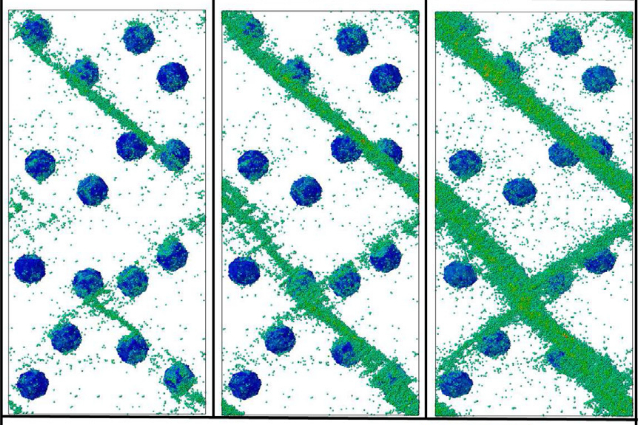
\includegraphics[width=5cm]{../Figures/Presentacion/nanoparticles_example.png}
	      \label{P:fg:B2Crystal}}
    \quad
      \subfloat[Nano vidrios \cite{Adibi13}]{
	      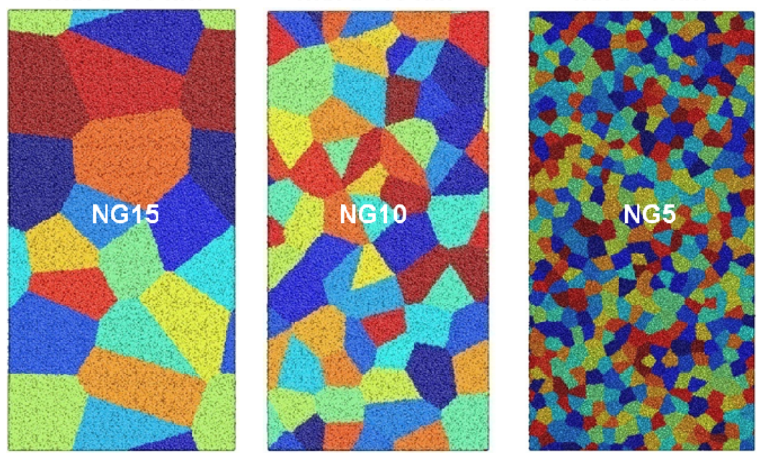
\includegraphics[width=5cm]{../Figures/Presentacion/nanoglass_example.png}
	      \label{P:fg:B2CrystalTest}}
    \end{tabular}
    \label{P:fg:B2CuZr_Formation}
  \end{figure} 
\end{frame}

\begin{frame}
\frametitle{Objetivos del estudio}
\vspace{0.5cm}
 \begin{itemize}
  \item Estabilidad térmica de las nanopartículas (difusión del material cristalino en la matriz amorfa).
  \item Impacto en el comportamiento mecánico de la muestra (cambios en curvas tensión-deformación)
  \item Distribución de la tensión de corte en la muestra.
 \end{itemize}
\end{frame}

\begin{frame}
 \frametitle{Detalles de la simulación}
 \vspace{0.5cm}
 \begin{itemize}
  \item Muestra original ya caracterizada: Cu$_{46}$Zr$_{54}$ - 160k átomos
  \item Condiciones de bordes periódicas en las tres dimensiones
  \item Nanopartículas: Esferas de 2 nm de radio de composición (a) Cu-FCC y (b) CuZr-B2
  \item La constante de red del cobre se establece en 0.3615 nm
  \item La estructura CuZr-B2 se genera ad-hoc para la simulación y da como resultado una constante de 0.3283 nm
  \item Velocidad de deformación de 10$^{9}$/s
 \end{itemize}
\end{frame}

\begin{frame}
 \frametitle{Preparación de cristal CuZr-B2}
 \only<1>{
  \begin{itemize}
    \item Cubo cristalino aislado de 15 celdas unitarias de ancho
    \item Constante de celda de 3.50 \AA{} \cite{inoue04}
    \item PBC en las tres dimensiones
    \item Minimizado de energía y relajación a presión cero.
    \item T$_{i}$ = 1100 K \cite{pauly10} (988 K $\leq$ T$_{B2}$ $\leq$ 1200 K)
    \item Se equilibra a P = 0 y T = T$_{B2}$ en 100 ps
    \item Recocido a T = T$_{B2}$ por 150 ps
    \item Enfriado rápido a 10$^{12}$ K/s hasta 300 K
  \end{itemize}
  }
  \only<2>{
  \begin{textblock*}{12cm}(0cm,3cm)
    \begin{table}[htp]
    \begin{center}
    \begin{tabular}{*{2}{c}}
    \hline
    Velocidad de enfriamiento [K/s] & 10$^{12}$ \\
    \hline
    Número de átomos & 6750 \\
    \hline
    Constante de celda [\AA] & 3.283 \\
    \hline
    Energía total (eV) & -34012.8 \\
    \hline
    Energía de cohesión (eV) & -5.04 \\
    \hline
    \end{tabular}
    \end{center}
    \end{table}
  \end{textblock*}
  
  \begin{textblock*}{12cm}(0cm,7cm) 
    \centering
      Parámetros obtenidos para el cristal CuZr (B2)
  \end{textblock*}
  }
  \only<3>{
    \begin{textblock*}{12.6cm}(-0.08cm,1.5cm) 
      \begin{figure}[htp]
	\centering
	\subfloat[Cristal]{
	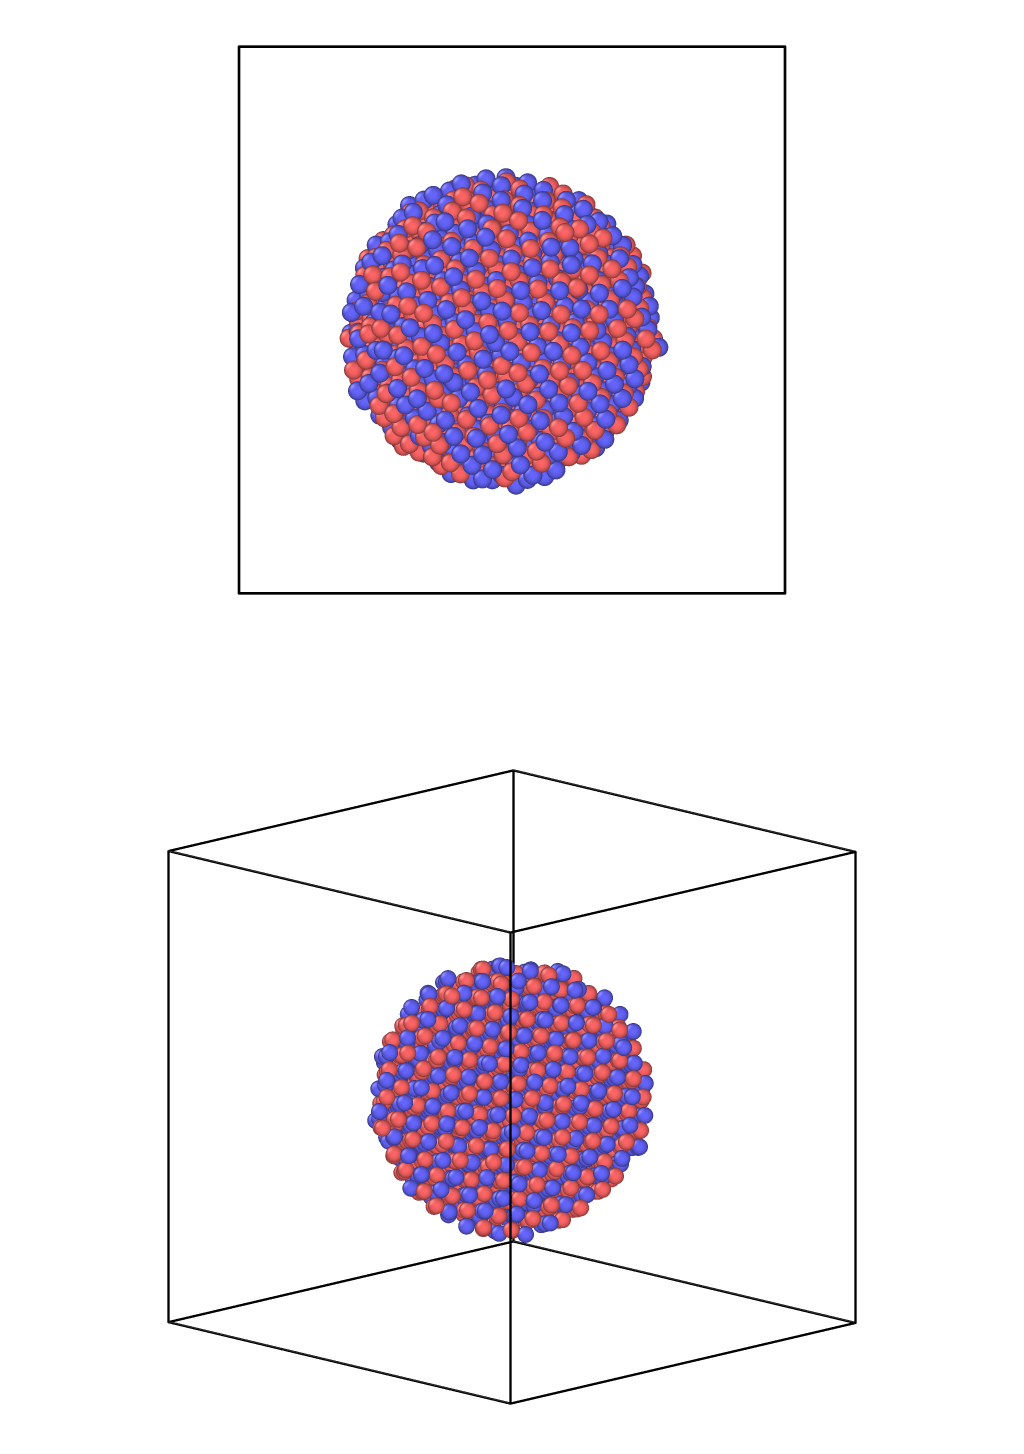
\includegraphics[height=5cm]{../Figures/Cap_4/B2_FreeBoundaries.png}}
	\subfloat[Energía de cohesión vs tiempo]{
	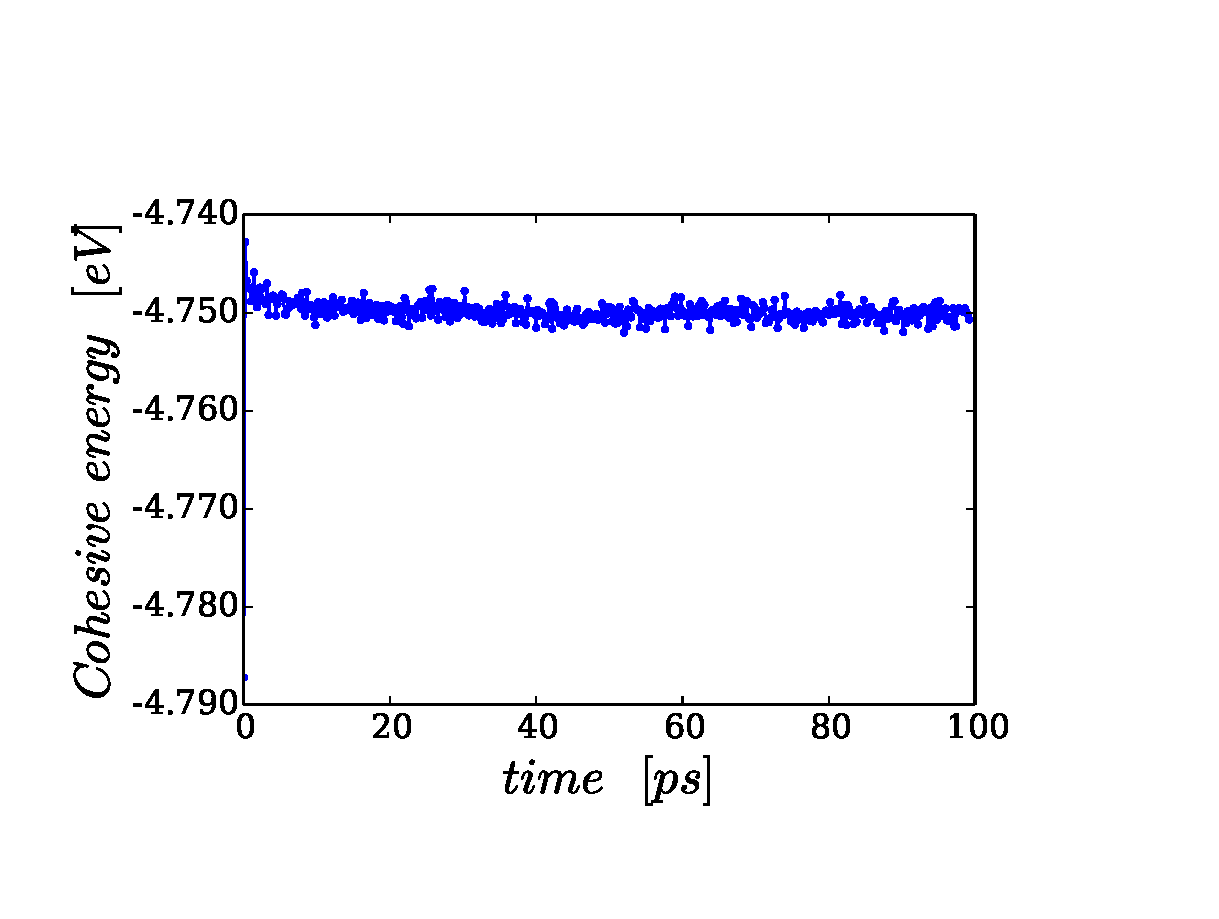
\includegraphics[width=6.3cm]{../Figures/Cap_4/B2CrystalTest_FreeBoundariesSphere.pdf}}
      \end{figure}
    \end{textblock*}
    \begin{textblock*}{10cm}(1.5cm,8.5cm) 
    \centering
      Verificación del cristal CuZr-B2
  \end{textblock*}
  }
\end{frame}

\begin{frame}
 \frametitle{Vista de la muestra preparada}
 
 \begin{textblock*}{12.6cm}(-0.08cm,1.5cm) 
     \begin{figure}[htp]
	\centering
	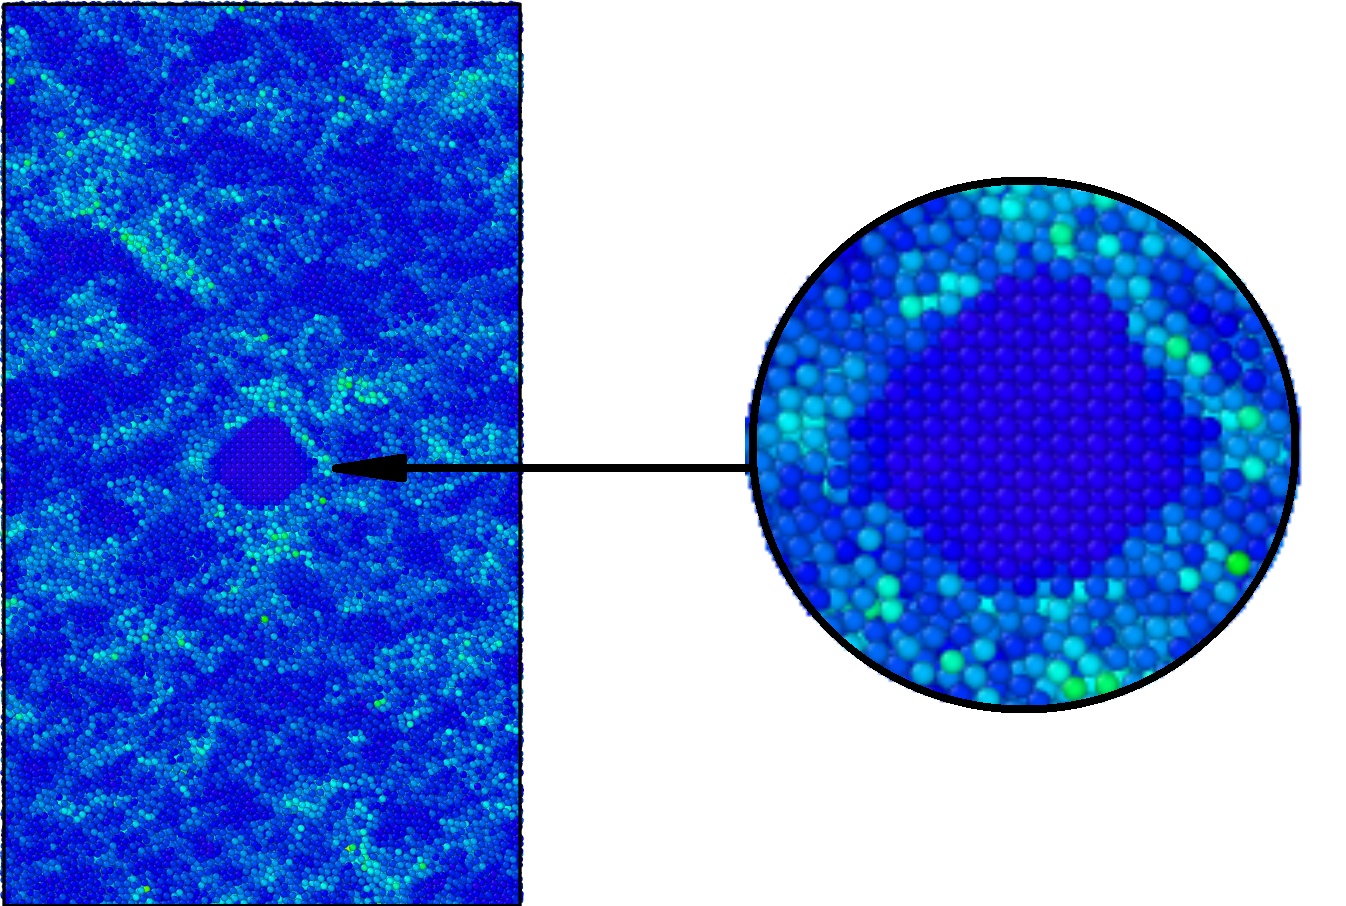
\includegraphics[height=6cm]{../Figures/Cap_4/NP_CloseUp_FCC.png}
      \end{figure}
  \end{textblock*}
 
\end{frame}

\begin{frame}
 \frametitle{Resultados}
 
 \begin{textblock*}{12.6cm}(-0.08cm,1.5cm) 
      \begin{figure}[htp]
	\centering
	\subfloat[Bajas Temperaturas]{
	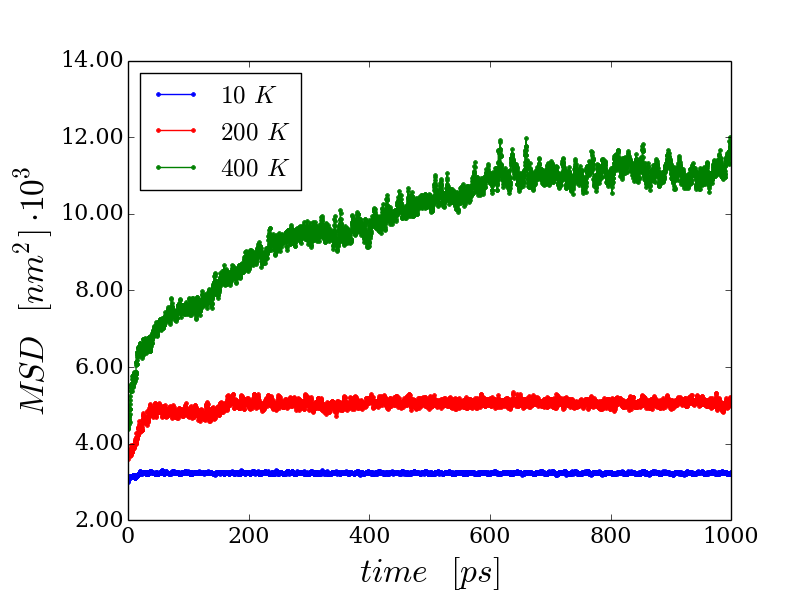
\includegraphics[width=6.3cm]{../Figures/Cap_4/msd10_400_FCC.png}}
	\subfloat[Altas Temperaturas]{
	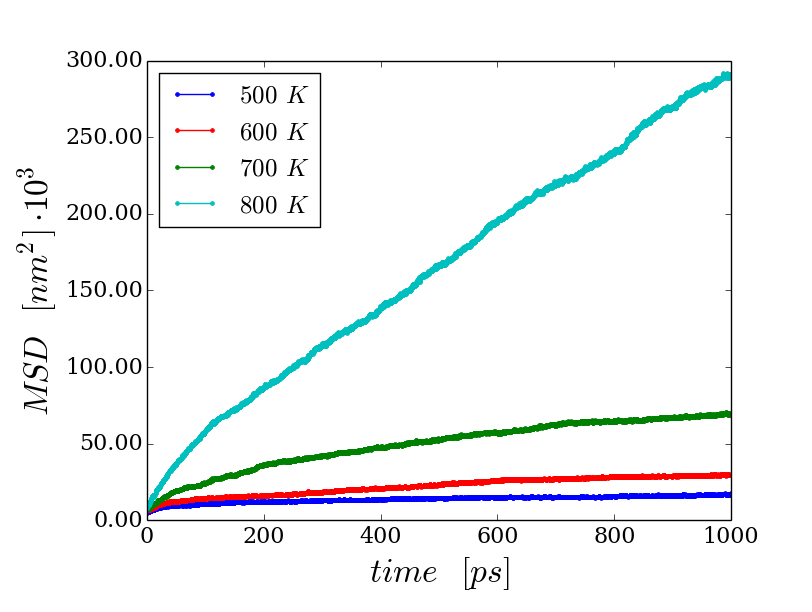
\includegraphics[width=6.3cm]{../Figures/Cap_4/msd500_800_FCC.png}}
      \end{figure}
    \end{textblock*}
    \begin{textblock*}{10cm}(1.5cm,8cm) 
    \centering
      Desplazamientos cuadráticos medios para la nanopartícula Cu-FCC
 \end{textblock*}
\end{frame}

\begin{frame}
 \frametitle{Resultados}
 
 \begin{textblock*}{12.6cm}(-0.08cm,1.5cm) 
      \begin{figure}[htp]
	\centering
	\subfloat[Bajas Temperaturas]{
	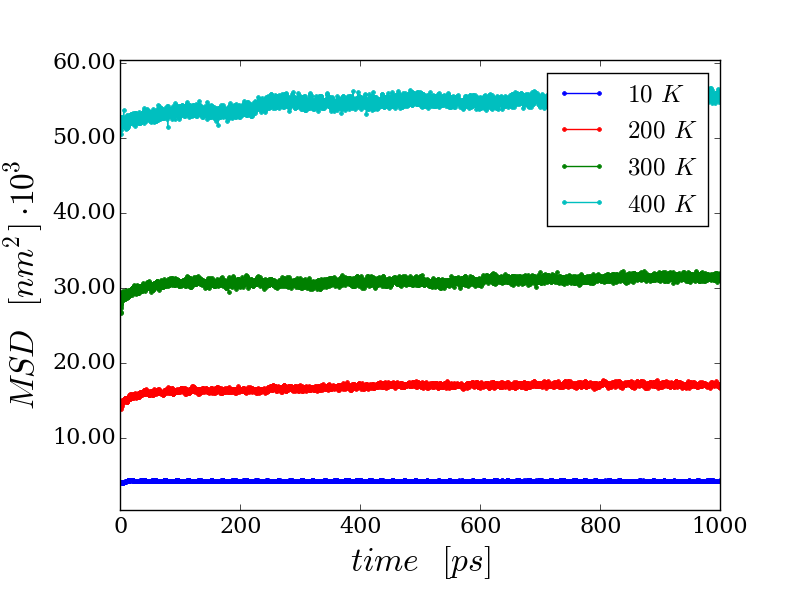
\includegraphics[width=6.3cm]{../Figures/Cap_4/msd10_400_B2.png}}
	\subfloat[Altas Temperaturas]{
	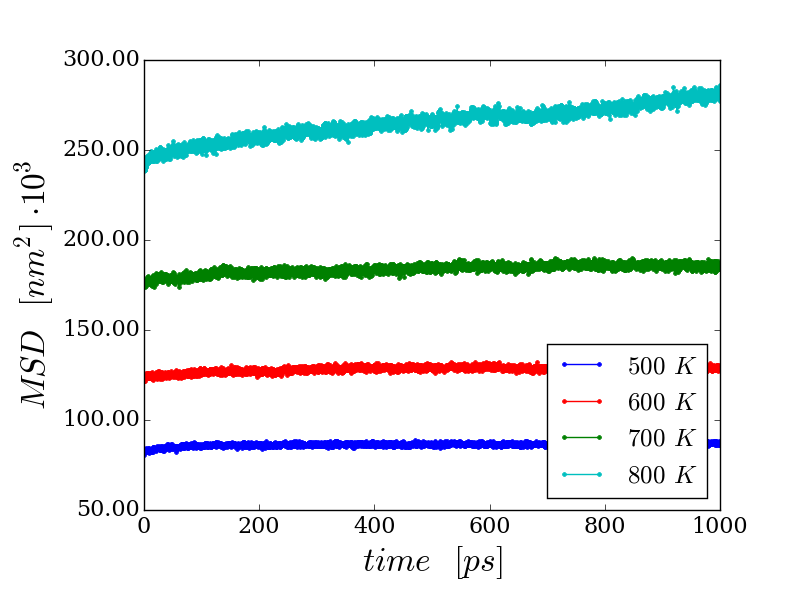
\includegraphics[width=6.3cm]{../Figures/Cap_4/msd500_800_B2.png}}
      \end{figure}
    \end{textblock*}
    \begin{textblock*}{10cm}(1.5cm,8cm) 
    \centering
      Desplazamientos cuadráticos medios para la nanopartícula CuZr-B2
 \end{textblock*}
\end{frame}

\begin{frame}
 \frametitle{Resultados}
 
  \begin{textblock*}{6.5cm}(-0.08cm,2cm) 
   \begin{figure}[htp]
    \centering
    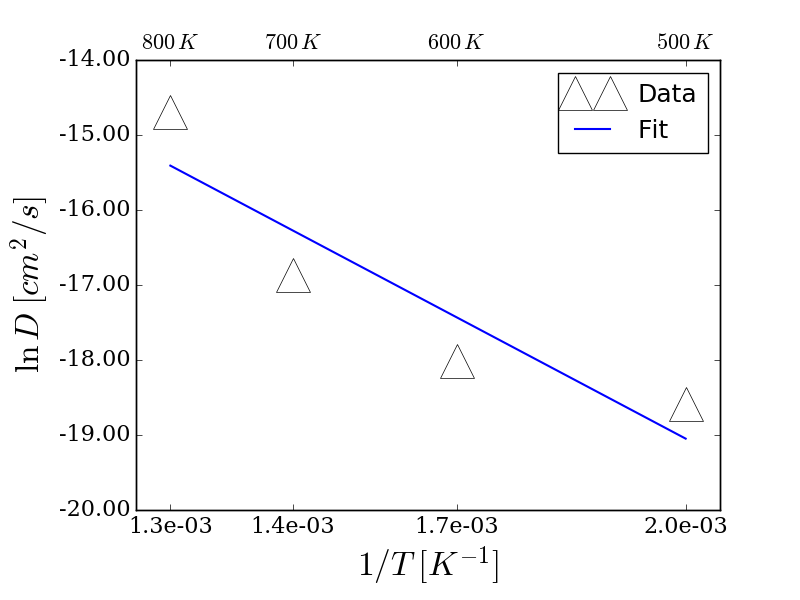
\includegraphics[width=6.3cm]{../Figures/Cap_4/FCCDiff_vs_temp_fit.png}
   \end{figure}
  \end{textblock*}
  \begin{textblock*}{10cm}(1.5cm,8cm) 
    \centering
    Difusividad en función de la temperatura para el caso Cu-FCC
  \end{textblock*}
  
  \begin{textblock*}{6cm}(6.5cm,3cm)
    Modelo usado para la regresión: \\
    $D = D_{0}\cdot \mathrm{e}^{\frac{-\Delta E}{k_{B} T}}$\\
    \vspace{0.5cm}
    Resultados de la regresión:
    \begin{table}[htp]
      \begin{center}
      \begin{tabular}{*{2}{c}}
      \hline
      $\Delta E$ [$eV$]& $-0,4182$ \\
      \hline
      D$_{0}$ [$\frac{nm^{2}}{ps}$] & $8,771\times 10^{-3}$\\
      \hline
      R$^{2}$ & 0.8399 \\
      \hline
      \end{tabular}
      \end{center}
      \end{table}    
  \end{textblock*} 
\end{frame}

\begin{frame}
 \frametitle{Carga uniaxial del BMG}
 \only<1>{
  \begin{textblock*}{12.6cm}(-0.08cm,1.5cm) 
      \begin{figure}[htp]
	\centering
	\subfloat[Tracci\'on]{
	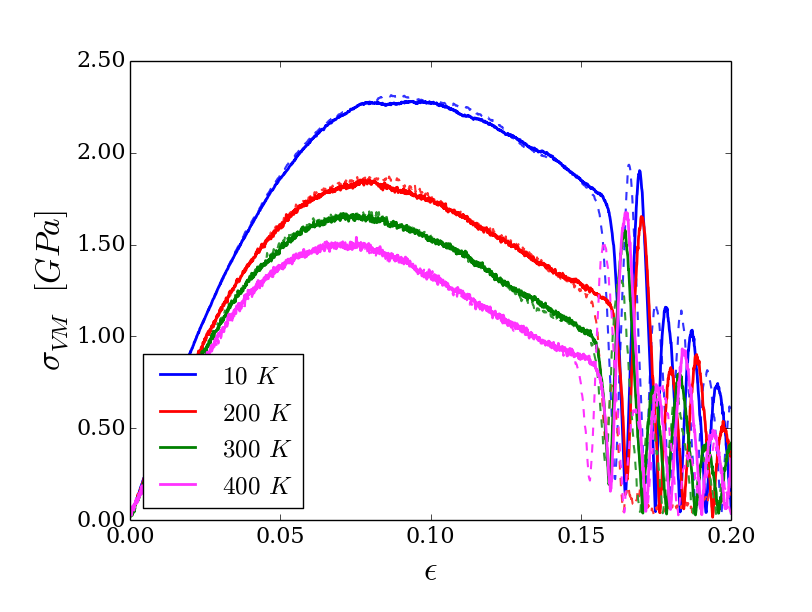
\includegraphics[width=6.3cm]{../Figures/Cap_4/stress_strain_tension_FCC_NoInc.png}}
	\subfloat[Compresi\'on]{
	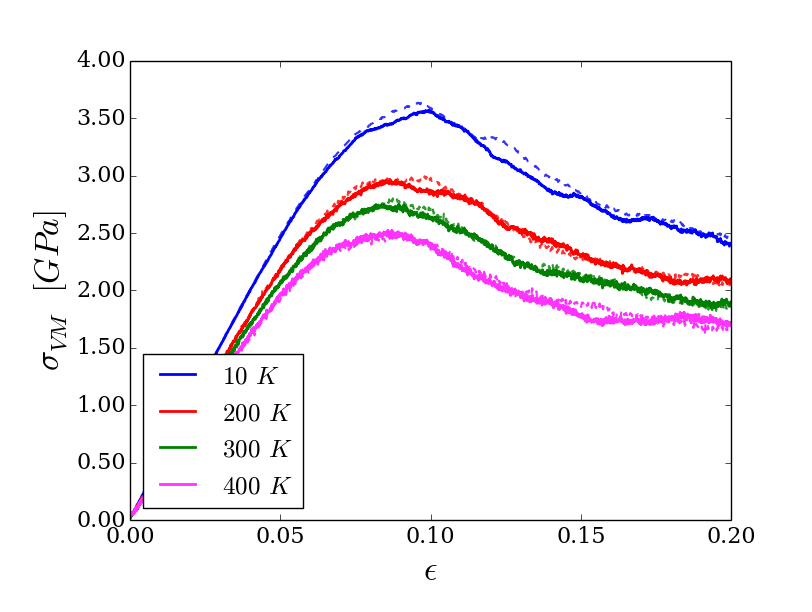
\includegraphics[width=6.3cm]{../Figures/Cap_4/stress_strain_compression_FCC_NoInc.png}}
      \end{figure}
    \end{textblock*}
    \begin{textblock*}{12cm}(0.5cm,8.5cm) 
    \centering
      Tensión de Von Mises vs deformación para el BMG sin inclusión (línea punteada) y una inclusión de Cu-FCC (línea sólida)
    \end{textblock*}
   }
   \only<2>{
    \begin{textblock*}{12.6cm}(-0.08cm,1.5cm) 
      \begin{figure}[htp]
	\centering
	\subfloat[Tracci\'on]{
	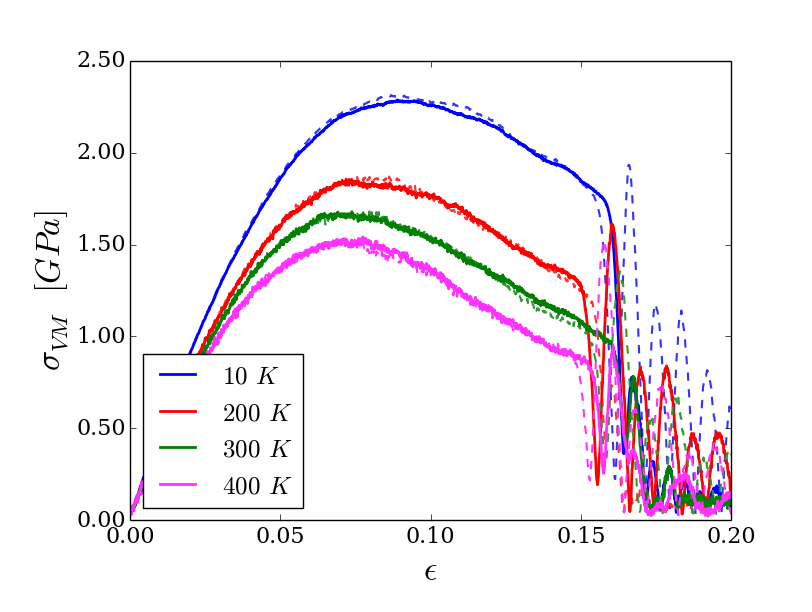
\includegraphics[width=6.3cm]{../Figures/Cap_4/stress_strain_tension_B2_NoInc.png}}
	\subfloat[Compresi\'on]{
	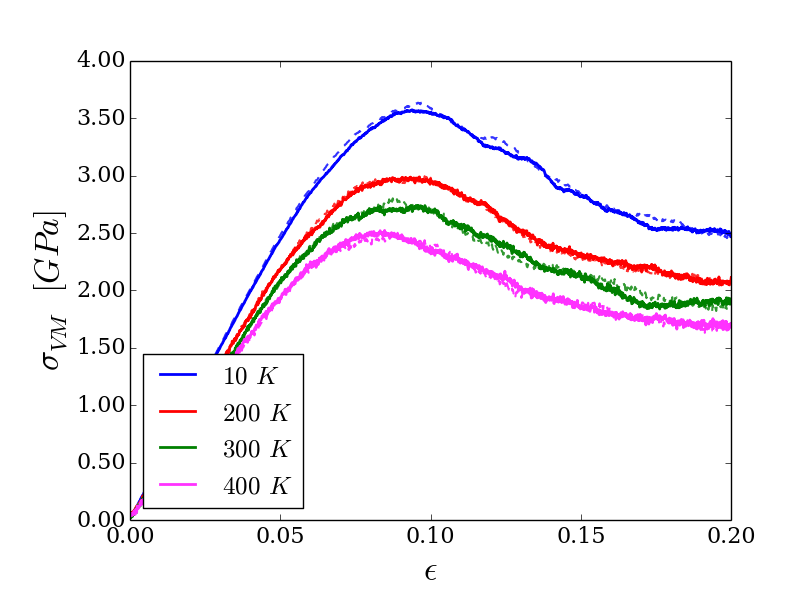
\includegraphics[width=6.3cm]{../Figures/Cap_4/stress_strain_compression_B2_NoInc.png}}
      \end{figure}
    \end{textblock*}
    \begin{textblock*}{12cm}(0.5cm,8.5cm) 
    \centering
      Tensión de Von Mises vs deformación para el BMG sin inclusión (línea punteada) y una inclusión de CuZr-B2 (línea sólida)
    \end{textblock*}
   }
\end{frame}


